\documentclass[12pt,a4paper]{report}

\usepackage[T1]{fontenc}
\usepackage[utf8]{inputenc}
\usepackage[margin=1in]{geometry}
\usepackage{graphicx}
\usepackage{amsmath,amssymb}
\usepackage{booktabs}
\usepackage{enumitem}
\usepackage{tikz}
\usetikzlibrary{arrows.meta,positioning,shapes.geometric,shapes.multipart,fit,calc}
\usepackage[hidelinks]{hyperref}
\usepackage{titlesec}
\usepackage{setspace}
\usepackage{float}

\setstretch{1.15}
\setlist{itemsep=3pt,topsep=4pt}
\titleformat{\chapter}[display]{\normalfont\huge\bfseries}{Chapter \thechapter}{12pt}{\Huge}
\titlespacing*{\chapter}{0pt}{-10pt}{20pt}

\begin{document}

%-------------------------------------------------------------
% Title page
%-------------------------------------------------------------
\begin{titlepage}
\centering
\vspace*{1cm}
{\Large \textbf{UCS503 -- Software Engineering}\par}
\vspace{1.5cm}
{\Huge \textbf{ClassLink}\par}
\vspace{0.4cm}
{\large A Cross-Platform BLE Proximity System for Classroom Attendance\par}
\vspace{2cm}

{\Large \textbf{Submitted by:}\par}
\vspace{0.4cm}
1024160102 \; Mahi Singh\\[2pt]
1024160109 \; Vrishank Nehru\\[2pt]
1024160123 \; Khagendra Saini\\[2pt]
1024160111 \; Vemula Manvi Smaran\\[6pt]
Group: 3P14 \quad BE Third Year, CSE

\vspace{1.5cm}
{\Large \textbf{Submitted to:}\par}
\vspace{0.4cm}
Miss Anushka

\vspace{1.2cm}
{\large \textbf{Mid-Semester Evaluation}\par}

\vfill
{\large Computer Science and Engineering Department\par}
Thapar Institute of Engineering and Technology, Patiala
\end{titlepage}

\tableofcontents
\clearpage

%-------------------------------------------------------------
\chapter{Introduction}

\section{Background and Context}
Manual attendance in a classroom is slow, easy to falsify, and produces no verifiable record of who was physically present. ClassLink addresses this by using Bluetooth Low Energy (BLE) proximity as the basis for attendance check-in: a teacher's device advertises a short-lived session code, and only student devices that are physically nearby can detect that signal and check in. This report documents the completed BLE discovery and proximity vertical slice of ClassLink, built as Phase~4 of a larger, contractually scoped system.

\section{Problem Statement}
The core technical problem is establishing reliable, cross-platform proximity-based discovery between a teacher device and multiple student devices using BLE alone, without relying on a backend, while working around platform-specific restrictions in how Android and iOS expose BLE advertisement data. A secondary problem is ensuring that proximity decisions are robust to noisy RSSI readings rather than reacting to a single stray packet.

\section{Project Objectives}
\begin{itemize}
  \item \textbf{Objective 1:} Implement a working BLE peripheral/central architecture in Flutter, where a teacher device advertises a session and student devices discover it directly, with no intermediate mesh or relay.
  \item \textbf{Objective 2:} Design a session-code transport that works identically from the student scanner's perspective on both Android and iOS, despite each platform exposing different subsets of BLE advertisement fields.
  \item \textbf{Objective 3:} Validate the proximity check against noisy real-world RSSI behaviour using a windowed, median-based threshold rather than a single-sample decision, and verify the implementation with unit tests and real-device builds.
\end{itemize}

%-------------------------------------------------------------
\chapter{Methodology and Design}

\section{System Architecture}
ClassLink's BLE vertical slice follows a direct peripheral--central model with no mesh or relay hop, matching the project's ``no BLE mesh in MVP'' design constraint.

\subsection{High-Level Design}
\begin{itemize}
  \item \textbf{Teacher device (BLE peripheral / advertiser):} starts a session, generates a 6-digit code, and broadcasts it over BLE.
  \item \textbf{Student device (BLE central / scanner):} scans for the ClassLink service UUID, collects RSSI samples over a fixed window, and once a valid proximity signal is confirmed, connects briefly to write a check-in payload containing the student's name and roll number.
  \item \textbf{Proximity decision:} the median of RSSI samples over a 4-second window is compared against a $-75$~dBm threshold, so a single noisy reading cannot trigger a false check-in.
\end{itemize}

\subsection{Technical Stack}
\begin{itemize}
  \item \textbf{Framework/Language:} Flutter/Dart, using native BLE peripheral and central APIs on Android and iOS.
  \item \textbf{Database:} None in this phase (see Section~\ref{sec:scope} on scope boundaries).
  \item \textbf{Tools:} \texttt{flutter analyze} for static analysis, Flutter's unit test framework, Apple's \texttt{devicectl} for physical iPhone deployment, and a Flutter release build for sideloaded Android APK distribution.
  \item \textbf{Libraries:} Platform BLE bindings for CoreBluetooth (iOS) and the Android Bluetooth LE stack.
\end{itemize}

\section{System Design Diagrams}
This section presents the system design using standard UML and structured-analysis views: a Use Case diagram showing the two actors and their interactions with the system, a Sequence diagram tracing the BLE advertising and check-in flow over time, a Class diagram of the core BLE components, a Component/Architecture diagram showing the current on-device scope alongside the planned backend, and a Data Flow Diagram (Level~0 and Level~1) showing how data moves through the system.

\subsection{Use Case Diagram}
\begin{figure}[H]
  \centering
  \includegraphics[width=0.85\textwidth]{figures/usecase.png}
  \caption{Use Case Diagram for ClassLink}
\end{figure}

\subsection{Sequence Diagram}
\begin{figure}[H]
  \centering
  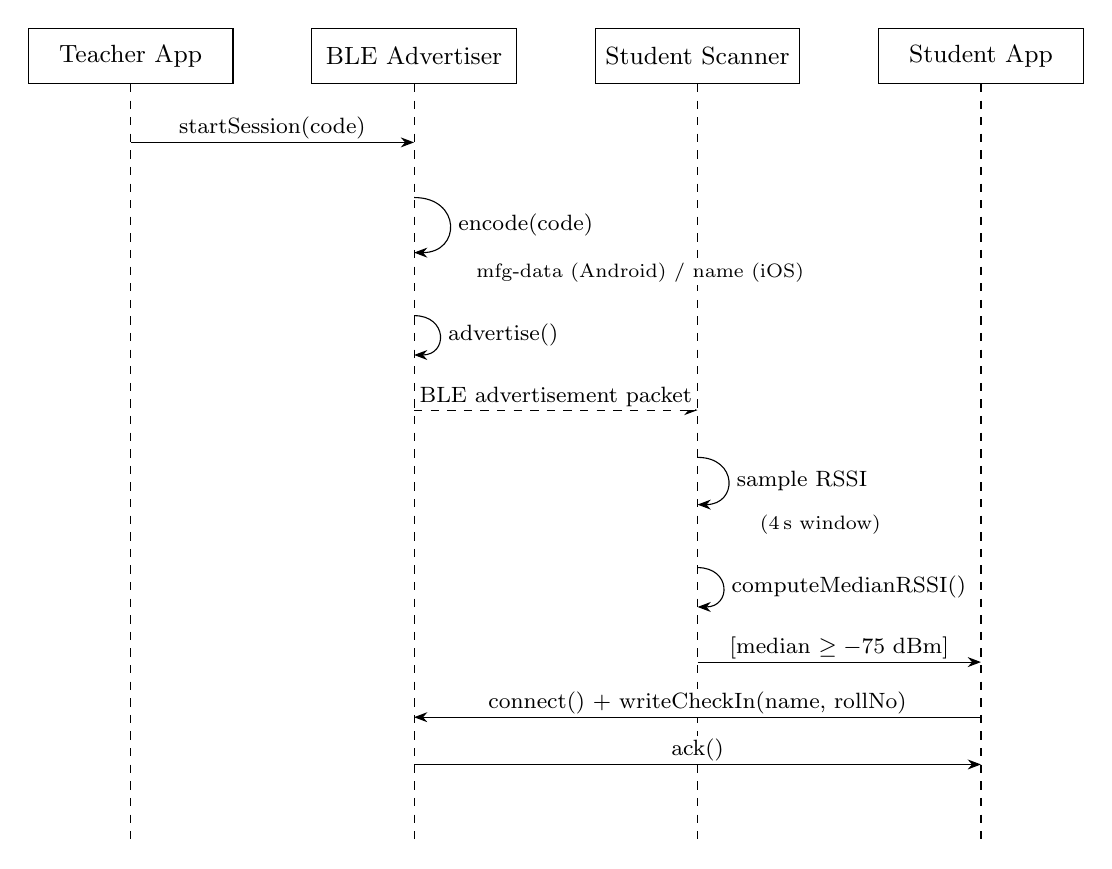
\begin{tikzpicture}[
    box/.style={draw,minimum width=2.6cm,minimum height=0.7cm,font=\small,align=center},
    msg/.style={-{Stealth},font=\footnotesize},
    life/.style={dashed}
  ]
    \node[box] (T) at (0,0) {Teacher App};
    \node[box] (A) at (3.6,0) {BLE Advertiser};
    \node[box] (S) at (7.2,0) {Student Scanner};
    \node[box] (U) at (10.8,0) {Student App};
    \foreach \n in {T,A,S,U} \draw[life] (\n.south) -- ++(0,-9.6);

    \draw[msg] (0,-1.1) -- node[above,fill=white,inner sep=1pt]{startSession(code)} (3.6,-1.1);
    \draw[msg] (3.6,-1.8) to[out=0,in=0,looseness=2.2] node[right,xshift=2pt,fill=white,inner sep=1pt]{\footnotesize encode(code)} (3.6,-2.5);
    \node[font=\scriptsize,anchor=west,fill=white,inner sep=1pt] at (4.35,-2.75) {mfg-data (Android) / name (iOS)};
    \draw[msg] (3.6,-3.3) to[out=0,in=0,looseness=2.2] node[right,xshift=2pt,fill=white,inner sep=1pt]{\footnotesize advertise()} (3.6,-3.8);
    \draw[msg,dashed] (3.6,-4.5) -- node[above,fill=white,inner sep=1pt]{BLE advertisement packet} (7.2,-4.5);
    \draw[msg] (7.2,-5.1) to[out=0,in=0,looseness=2.2] node[right,xshift=2pt,fill=white,inner sep=1pt]{\footnotesize sample RSSI} (7.2,-5.7);
    \node[font=\scriptsize,anchor=west,fill=white,inner sep=1pt] at (7.95,-5.95) {(4\,s window)};
    \draw[msg] (7.2,-6.5) to[out=0,in=0,looseness=2.2] node[right,xshift=2pt,fill=white,inner sep=1pt]{\footnotesize computeMedianRSSI()} (7.2,-7.0);
    \draw[msg] (7.2,-7.7) -- node[above,fill=white,inner sep=1pt]{[median $\ge -75$ dBm]} (10.8,-7.7);
    \draw[msg] (10.8,-8.4) -- node[above,fill=white,inner sep=1pt]{connect() + writeCheckIn(name, rollNo)} (3.6,-8.4);
    \draw[msg] (3.6,-9.0) -- node[above,fill=white,inner sep=1pt]{ack()} (10.8,-9.0);
  \end{tikzpicture}
  \caption{Sequence Diagram: BLE Advertising and Check-in Flow}
\end{figure}

\subsection{Class Diagram}
\begin{figure}[H]
  \centering
  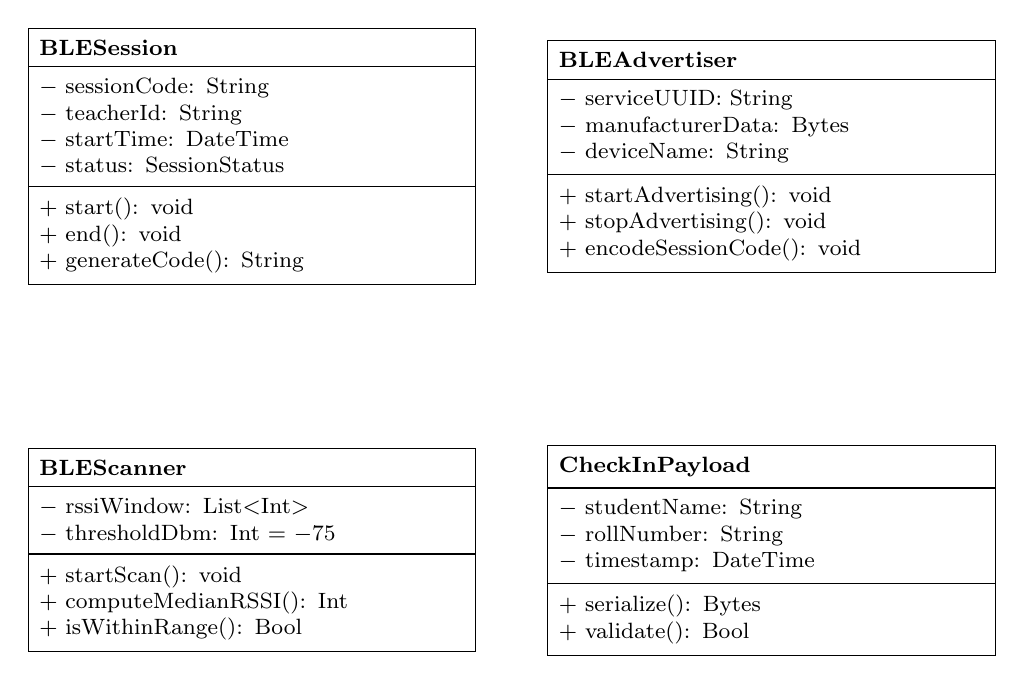
\begin{tikzpicture}[
    cls/.style={draw,rectangle split,rectangle split parts=3,font=\footnotesize,
                text width=5.4cm,align=left,inner sep=4pt}
  ]
    \node[cls] (s) at (0,0) {\textbf{BLESession}
      \nodepart{two}$-$ sessionCode: String\\$-$ teacherId: String\\$-$ startTime: DateTime\\$-$ status: SessionStatus
      \nodepart{three}+ start(): void\\+ end(): void\\+ generateCode(): String};
    \node[cls] (a) at (6.6,0) {\textbf{BLEAdvertiser}
      \nodepart{two}$-$ serviceUUID: String\\$-$ manufacturerData: Bytes\\$-$ deviceName: String
      \nodepart{three}+ startAdvertising(): void\\+ stopAdvertising(): void\\+ encodeSessionCode(): void};
    \node[cls] (b) at (0,-5.0) {\textbf{BLEScanner}
      \nodepart{two}$-$ rssiWindow: List$<$Int$>$\\$-$ thresholdDbm: Int = $-75$
      \nodepart{three}+ startScan(): void\\+ computeMedianRSSI(): Int\\+ isWithinRange(): Bool};
    \node[cls] (c) at (6.6,-5.0) {\textbf{CheckInPayload}
      \nodepart{two}$-$ studentName: String\\$-$ rollNumber: String\\$-$ timestamp: DateTime
      \nodepart{three}+ serialize(): Bytes\\+ validate(): Bool};
  \end{tikzpicture}
  \caption{Class Diagram: Core BLE Components}
\end{figure}

\subsection{Component / Architecture Diagram}
\begin{figure}[H]
  \centering
  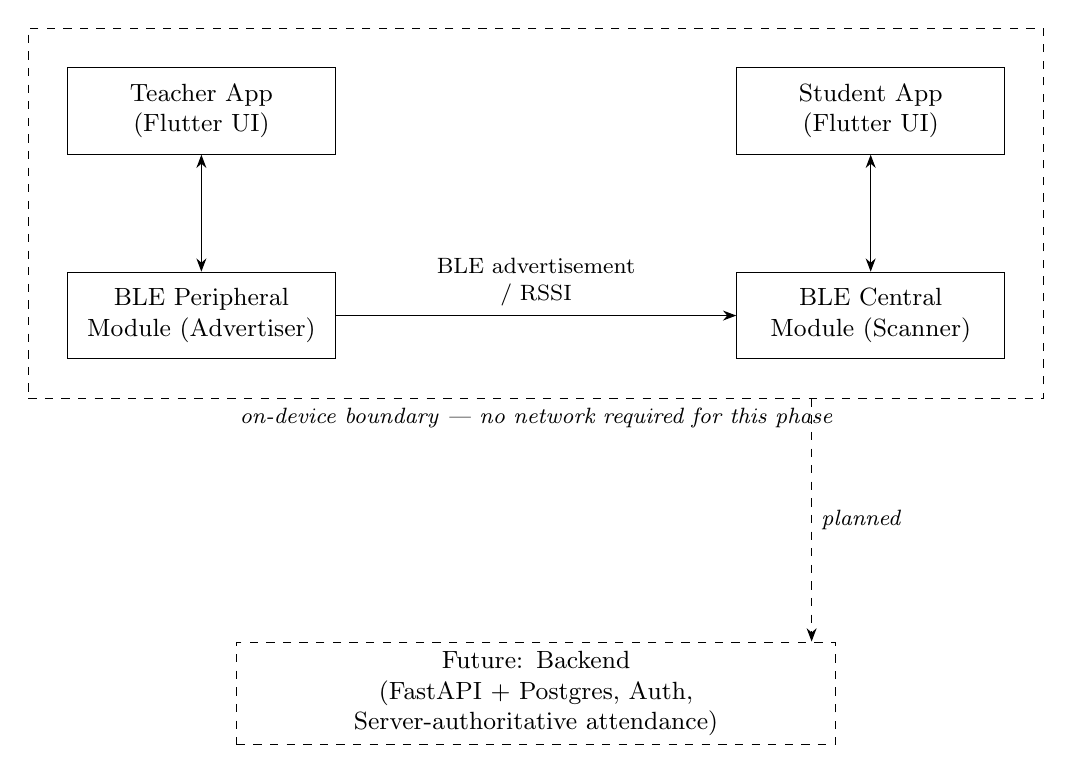
\begin{tikzpicture}[
    comp/.style={draw,minimum width=3.4cm,minimum height=1.1cm,align=center,font=\small},
    arr/.style={{Stealth}-{Stealth}}
  ]
    \node[comp] (ta) at (0,0) {Teacher App\\(Flutter UI)};
    \node[comp] (sa) at (8.5,0) {Student App\\(Flutter UI)};
    \node[comp] (bp) at (0,-2.6) {BLE Peripheral\\Module (Advertiser)};
    \node[comp] (bc) at (8.5,-2.6) {BLE Central\\Module (Scanner)};
    \draw[arr] (ta) -- (bp);
    \draw[arr] (sa) -- (bc);
    \draw[-{Stealth}] (bp) -- node[above,font=\footnotesize,align=center]{BLE advertisement\\/ RSSI} (bc);
    \node[draw,dashed,fit=(ta)(sa)(bp)(bc),inner sep=14pt,
          label={[font=\footnotesize\itshape]below:on-device boundary --- no network required for this phase}] (bound) {};
    \node[comp,dashed,minimum width=7.6cm,text width=7.2cm] (be) at (4.25,-7.4) {Future: Backend\\(FastAPI + Postgres, Auth, Server-authoritative attendance)};
    \draw[dashed,-{Stealth}] ($(bound.south)+(3.5,0)$) -- node[right,font=\footnotesize\itshape]{planned} ($(be.north)+(3.5,0)$);
  \end{tikzpicture}
  \caption{High-Level Component Architecture}
\end{figure}

\subsection{Data Flow Diagram}
\begin{figure}[H]
  \centering
  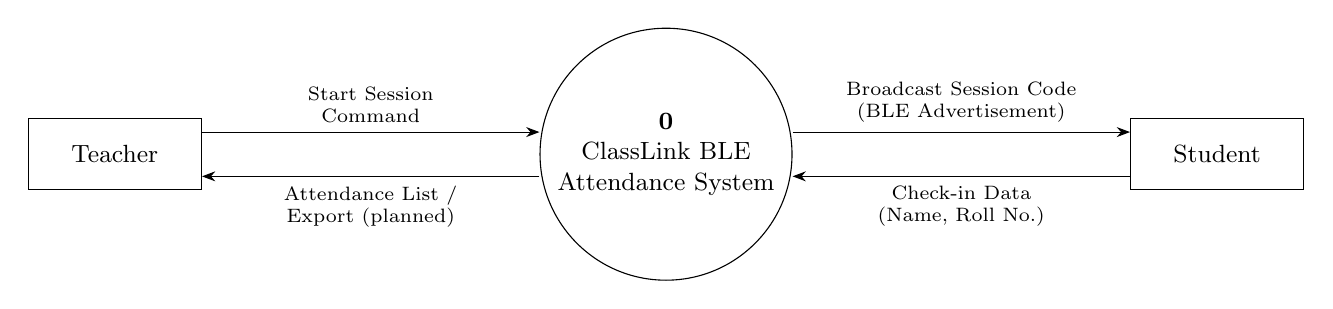
\begin{tikzpicture}[
    ext/.style={draw,minimum width=2.2cm,minimum height=0.9cm,font=\small},
    proc/.style={draw,circle,align=center,font=\small,inner sep=2pt},
    flow/.style={-{Stealth},font=\scriptsize,align=center}
  ]
    \node[ext] (t) at (-7,0) {Teacher};
    \node[ext] (s) at (7,0) {Student};
    \node[proc,minimum size=3.2cm] (p) at (0,0) {\textbf{0}\\ClassLink BLE\\Attendance System};
    \draw[flow] ([yshift=8pt]t.east) -- node[above]{Start Session\\Command} ([yshift=8pt]p.west |- t.east);
    \draw[flow] ([yshift=-8pt]p.west |- t.east) -- node[below]{Attendance List /\\Export (planned)} ([yshift=-8pt]t.east);
    \draw[flow] ([yshift=8pt]p.east |- s.west) -- node[above]{Broadcast Session Code\\(BLE Advertisement)} ([yshift=8pt]s.west);
    \draw[flow] ([yshift=-8pt]s.west) -- node[below]{Check-in Data\\(Name, Roll No.)} ([yshift=-8pt]p.east |- s.west);
  \end{tikzpicture}
  \caption{Data Flow Diagram --- Level 0 (Context Diagram)}
\end{figure}

\begin{figure}[H]
  \centering
  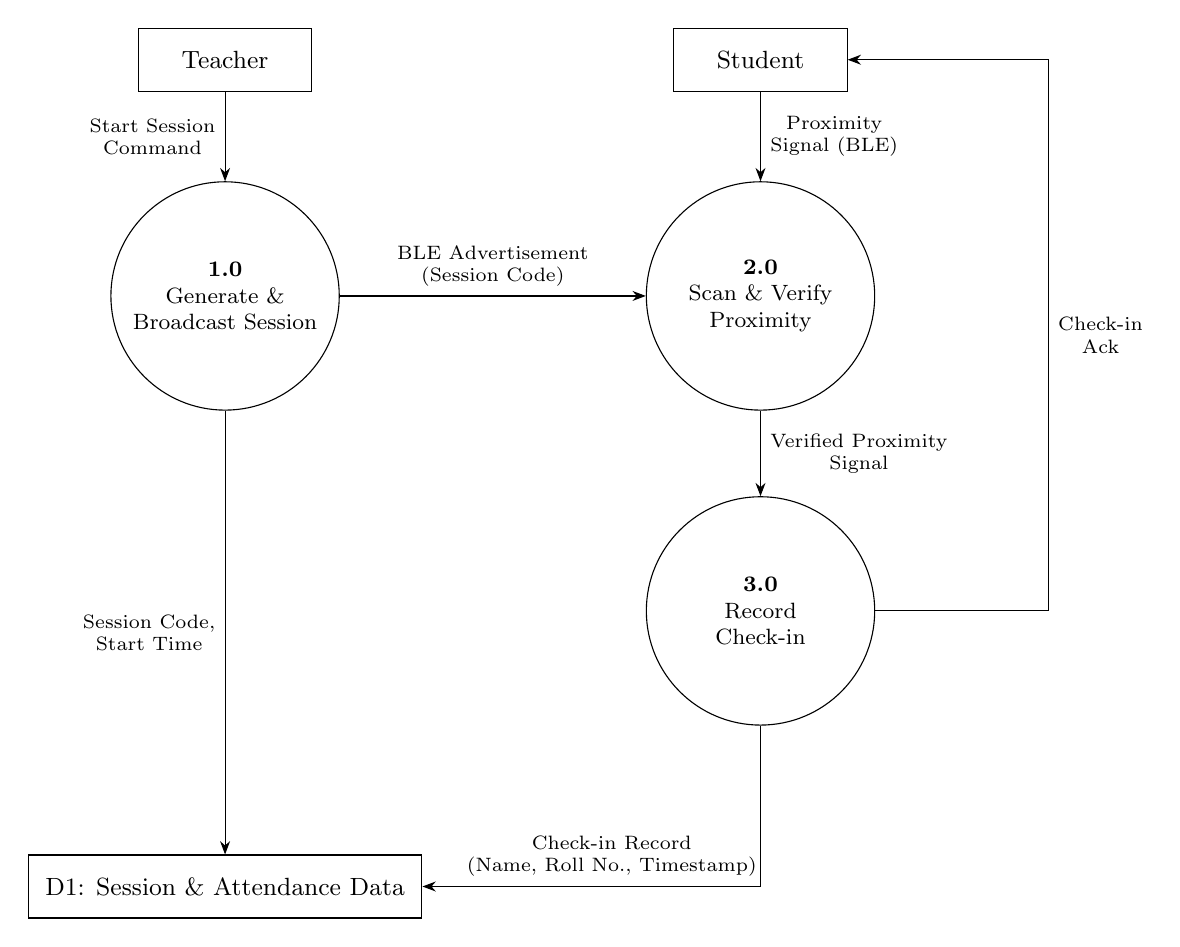
\begin{tikzpicture}[
    ext/.style={draw,minimum width=2.2cm,minimum height=0.8cm,font=\small},
    proc/.style={draw,circle,align=center,font=\footnotesize,minimum size=2.9cm,inner sep=1pt},
    store/.style={draw,minimum width=5cm,minimum height=0.8cm,font=\small},
    flow/.style={-{Stealth},font=\scriptsize,align=center}
  ]
    \node[ext] (t) at (0,0) {Teacher};
    \node[proc] (p1) at (0,-3) {\textbf{1.0}\\Generate \&\\Broadcast Session};
    \node[proc] (p2) at (6.8,-3) {\textbf{2.0}\\Scan \& Verify\\Proximity};
    \node[proc] (p3) at (6.8,-7) {\textbf{3.0}\\Record\\Check-in};
    \node[store] (d1) at (0,-10.5) {D1: Session \& Attendance Data};
    \node[ext] (s) at (6.8,0) {Student};

    \draw[flow] (t) -- node[left]{Start Session\\Command} (p1);
    \draw[flow] (p1) -- node[above]{BLE Advertisement\\(Session Code)} (p2);
    \draw[flow] (s) -- node[right]{Proximity\\Signal (BLE)} (p2);
    \draw[flow] (p2) -- node[right]{Verified Proximity\\Signal} (p3);
    \draw[flow] (p1.south) -- node[left]{Session Code,\\Start Time} (d1.north);
    \draw[flow] (p3.south) |- node[pos=0.72,above]{Check-in Record\\(Name, Roll No., Timestamp)} (d1.east);
    \draw[flow] (p3.east) -- ++(2.2,0) |- node[pos=0.25,right]{Check-in\\Ack} (s.east);
  \end{tikzpicture}
  \caption{Data Flow Diagram --- Level 1}
\end{figure}

\section{Implementation Details}

\subsection{Module 1: Cross-Platform BLE Advertising}
The central engineering problem solved in this phase was cross-platform BLE advertising. iOS's CoreBluetooth framework silently drops manufacturer-specific data from BLE advertisements when the app is in the background or, in practice, restricts advertisement content to a local device name and service UUIDs only; Android has no equivalent restriction. Because the original design encoded the session code as manufacturer-specific data, it worked on Android but silently failed on iOS with no runtime error, making the defect difficult to detect without cross-platform testing.

The fix was a platform-adaptive transport:
\begin{itemize}
  \item \textbf{Android:} the session code is sent as 10 bytes of manufacturer-specific data alongside the service UUID. This fits the legacy 31-byte BLE advertisement limit exactly: 3 bytes of flags, 18 bytes for the 128-bit service UUID, and 10 bytes of manufacturer data.
  \item \textbf{iOS:} the session code is instead embedded in the advertised local device name, formatted as \texttt{CL<6-digit-code>} (e.g.\ \texttt{CL042917}). This is deliberately not used on Android, since setting the advertised name there renames the phone's actual Bluetooth adapter.
  \item \textbf{Scanner logic:} the student-side scanner checks manufacturer data first, then falls back to parsing the advertised device name, so a single scanner implementation can discover either an Android or an iOS teacher device without knowing in advance which platform is advertising.
\end{itemize}

Two further defects were identified and fixed during this work. First, the original advertisement omitted the service UUID that the scanner itself filtered on, which made discovery impossible on both platforms. Second, BLE commands were being issued before the Bluetooth stack reported a \texttt{poweredOn} state, which CoreBluetooth silently rejects on a fresh app launch; this was fixed with a wait-and-timeout guard that surfaces specific, actionable errors (Bluetooth off, unauthorized, or unsupported) instead of failing silently.

\subsection{Module 2: Android 12+ Permission Handling}
A second defect was found in how the app requested runtime permissions on Android. The app originally requested \texttt{ACCESS\_FINE\_LOCATION} as a hard requirement on all Android versions in order to perform BLE scanning. On Android~12 and above, the manifest correctly declares \texttt{BLUETOOTH\_SCAN} with the \texttt{neverForLocation} flag, since the app only uses RSSI for proximity and never derives physical location. However, that flag also causes the OS to auto-deny any accompanying location permission request, which would have silently blocked the entire check-in flow on any modern Android phone. This was fixed by treating Bluetooth permissions as the hard requirement on Android~12+, and location permission as a best-effort request that is only relevant on pre-Android~12 devices.

\subsection{Scope Boundaries}\label{sec:scope}
This proof-of-concept intentionally implements only Phase~4 (the BLE vertical slice) of a larger system defined in the project's own engineering contract. The following are deliberately out of scope for this phase, and are noted here so the evaluation scope is unambiguous:
\begin{itemize}
  \item No backend (FastAPI) and no database (Supabase/Postgres); no Row-Level Security.
  \item No authentication, no roles, and no classroom/enrollment model.
  \item No rotating session tokens, no server-issued challenges, and no cryptographic device binding or signing.
  \item No biometric authentication step.
  \item Attendance decisions currently happen client-side; the project's contract requires all attendance mutation to be server-authoritative in the final system. This is a known, tracked gap rather than an oversight.
  \item No audit logging and no manual-correction workflow. CSV export UI exists on-screen but is not yet wired to a real backend.
\end{itemize}

%-------------------------------------------------------------
\chapter{Results and Evaluation}

\section{Testing Methodology}
\begin{itemize}
  \item \textbf{Unit Testing:} 16 unit tests were written and pass, including 5 tests added specifically to cover the session-code transport: manufacturer-data round-trip, iOS name round-trip, rejection of malformed or unrelated advertised names, and correctness of the 31-byte advertisement budget.
  \item \textbf{Static Analysis:} \texttt{flutter analyze} reports no issues on the current codebase.
  \item \textbf{Real-Device Testing:} the app was installed and launched on a physical iPhone using a release build via \texttt{devicectl} (chosen because wireless \texttt{flutter run} debugging proved unreliable), and a real release APK (45~MB, containing compiled \texttt{classes.dex}) was built and verified for Android.
  \item \textbf{Cross-Platform Testing:} a two-phone cross-platform test (iPhone-as-teacher with Android-as-student, and the reverse role assignment) is the next concrete milestone and had not been formally executed and recorded at the time of writing; this is flagged here as the immediate next validation step, to be captured with timestamped screenshots.
\end{itemize}

\section{Performance Metrics}
\begin{table}[H]
  \centering
  \begin{tabular}{@{}ll@{}}
    \toprule
    \textbf{Metric} & \textbf{Result} \\
    \midrule
    Unit tests passing & 16 / 16 \\
    Static analysis issues & 0 \\
    Proximity window & 4\,s (median RSSI) \\
    Proximity threshold & $-75$\,dBm \\
    Android advertisement budget used & 31 / 31 bytes \\
    Android release APK size & 45\,MB \\
    \bottomrule
  \end{tabular}
  \caption{Testing and Build Results Summary}
\end{table}

\section{Analysis}
The primary objective of this phase --- proving that a single BLE scanner implementation can reliably discover both an Android and an iOS teacher device --- was met.

The iOS/CoreBluetooth advertisement-data restriction was not documented clearly enough in the BLE library's own documentation to anticipate in advance; it was discovered empirically by observing that discovery worked on Android but failed silently on iOS, which is itself a notable finding for a BLE-based system built across both mobile platforms. The windowed, median-based proximity check was chosen specifically to avoid false check-ins from single noisy RSSI samples, and the Android~12+ permission fix removed a defect that would otherwise have silently blocked check-in on the majority of current Android devices.

The main outstanding challenge is that the two-phone, cross-platform, real-world check-in has not yet been formally executed and recorded, even though each platform has been independently verified in isolation (unit tests, static analysis, and single-device real hardware runs). This is the immediate next step before this vertical slice can be considered fully validated end-to-end.

%-------------------------------------------------------------
\chapter{Conclusion}

\section{Summary of Work}
This report presented ClassLink's completed BLE discovery and proximity vertical slice: a teacher device advertises a session over BLE, and student devices discover it and check in based on a windowed proximity check, using a session-code transport that adapts to each platform's BLE advertisement constraints. This represents Phase~4 of a larger planned system and was validated through unit testing, static analysis, and real-device builds on both Android and iOS.

\section{Key Findings}
\begin{itemize}
  \item \textbf{Finding 1:} iOS's CoreBluetooth framework restricts BLE advertisement content to a local device name and service UUIDs, silently dropping manufacturer-specific data; this required a platform-adaptive session-code transport rather than a single shared encoding.
  \item \textbf{Finding 2:} Android's \texttt{neverForLocation} flag on \texttt{BLUETOOTH\_SCAN}, while correct for an app that only uses RSSI proximity, causes the OS to auto-deny any accompanying location permission request on Android~12+, which would have silently blocked the entire check-in flow if location had remained a hard requirement.
  \item \textbf{Finding 3:} a single, unified scanner implementation can support discovery of either platform's teacher device by checking manufacturer data first and falling back to parsing the advertised device name, avoiding the need for platform-specific scanner logic on the student side.
\end{itemize}

\section{Future Work and Recommendations}
\begin{itemize}
  \item Execute and formally record the two-phone, cross-platform check-in test (iPhone teacher with Android student, and the reverse), with timestamped screenshots.
  \item Build the server-authoritative backend (FastAPI with a Supabase/Postgres database and Row-Level Security) so attendance mutation no longer happens client-side.
  \item Add authentication, roles, and a classroom/enrollment model.
  \item Introduce rotating session tokens, server-issued challenges, and cryptographic device binding or signing, in place of the current static 6-digit code.
  \item Add a biometric authentication step, audit logging, a manual-correction workflow, and wire the existing CSV export UI to a real backend.
\end{itemize}

\section{Final Remarks}
This phase deliberately targeted the hardest and most platform-fragile part of ClassLink --- BLE discovery and proximity detection under real operating-system constraints --- before investing in the server-authoritative security model that the project's engineering contract ultimately requires. With that vertical slice working and tested, the project is well positioned to move on to the backend, authentication, and security work that remains.

\end{document}
